\documentclass{acmsiggraph}

% \usepackage{mathptmx}
\usepackage{graphicx}
% \usepackage{epsfig}
% \usepackage{amsmath,amscd,amssymb}

% \newtheorem{theorem}{Theorem}[section]
% \newtheorem{proposition}[theorem]{Proposition}
% \newtheorem{definition}[theorem]{Definition}
% \newtheorem{lemma}[theorem]{Lemma}
% \newtheorem{corollary}[theorem]{Corollary}
% \newtheorem{remark}[theorem]{Remark}

\usepackage{parskip}

% \onlineid{papers\_0142} % REVIEW

% \acmformat{cameraready} TODO

\title{Garland and Heckbert’s Algorithm for Surface Simplification in Python 3.9.0}

\author{Jesse Chick\thanks{\small\texttt{e-mail: \{chickj,wilsono\}@oregonstate.edu}}\\ Oregon State University
\and Odyssey Wilson$^{\ast}$ \\
Oregon State University}

\keywords{python, suface simplication}

%%%%%% START OF THE PAPER %%%%%%

\begin{document} % TODO revise tense

\maketitle

% SECTION Abstract
\begin{abstract}
% \copyrightspace
Michael Garland and Paul S. Heckbert of Carnegie Mellon University discuss
their method of three dimensional surface simplification in their paper
“Surface Simplification Using Quadric Error Metrics”. By strategically deciding
on pairs of vertices to contract together and storing error approximations in
4x4 quadric matrices, Garland and Heckbert are able to create approximations
quickly and accurately while adding support for non-manifold objects. We 
developed a Python implementation of Garland and Heckbert’s algorithm to create
quadric error matrices for each vertex, determine edges that are eligible to
contract, calculate each edge’s contraction cost, iteratively contracting each
edge from lowest to highest cost, and updating the costs for edges that are
affected.
\end{abstract}
% !SECTION Abstract

% \keywordlist TODO have Odyssey do this

% SECTION Introduction
\section{Introduction}
% \label{sec:intro}
Original models in computer graphics applications tend to be created at high
resolutions to adequately represent the object being modeled. These complex
models can often be approximated into simpler versions to be used in situations
like rendering an object from a distance or visualizing a model where the
topology of the object is not a priority. Rather than having to create these
approximations by hand, Garland and Heckbert’s algorithm provides a way for
surfaces to be simplified down to these approximations automatically using one
of two methods of constraint. The first is a desired number of faces that the
approximation should possess and the second is a maximum error threshold where
no two vertices with a cost higher than the threshold should be contracted. Our
implementation takes a desired number of edges to be contracted and performs
those contractions iteratively from lowest to highest cost.

Garland and Heckbert specify the three primary goals of their algorithm as
efficiency, quality and generality. Naturally we attempted to embody these
ideas in our own implementation, minor discrepancies notwithstanding.

\subsection{Efficiency}
Garland and Heckbert explain their implementation is efficient in both the
aspect of time and space. They are able to, for example, approximate a 70,000
face object down to 100 faces in 15 seconds. We did not attempt to approximate
any models quite as complicated, but our implementation is still fast,
especially for having implemented it in python. For example, the original
panther model has 570 faces and we are able to perform the maximum 283
contractions practically instantly. In terms of space, Garland and Heckbert
take pride in their ability to compact error approximation into 10 floating
point numbers by using the quadric error matrices which our implementation
mimics.

\subsection{Quality}
Maintaining an original model’s primary features after approximation is
something that Garland and Heckbert deem of high importance and we attempt to
achieve this as well. This can be seen in the panther model in the results
section where after applying 220 contractions the approximation still has a
distinguishable head, body, tail, and set of legs.

\subsection{Generality}
To achieve their goal of supporting non-manifold objects, Garland and Heckbert
introduce the idea of aggregation which they use as a title for the process of
connecting sections of the original model that were previously disconnected.
For example, if a mesh of an animal has a hole to represent its eye, the
algorithm could decide to close this hole. Since we followed their algorithm
outline in our implementation, our code is also able to be run on a large
variety of shapes.
% !SECTION Introduction

% SECTION Previous Work
\section{Previous Work}
% \label{sec:previous_work}
Garland and Heckbert released their paper in 1997 and lots of work in surface
simplification has been done since then. Prior to Garland and Heckbert’s work,
there were following three standard methods of approximating models:

\subsection{Vertex Decimation}
An iterative method of choosing a vertex to remove, removing all faces
connected to it, and re-triangulating to fill the resulting gap. This method,
according to Garland and Heckbert, does a satisfactory job as far as efficiency
and quality, but is not versatile enough. The re-triangulation prevents support
for non-manifold edges however it does preserve the original model’s topography
which can be important in situations like medical imaging.

\subsection{Vertex Clustering}
Begins by encapsulating the original model in a bounding box and dividing it up
into a grid with specific cell sizes. Then, all vertices within each cell are
contracted into a single vertex and all affected faces are updated. While this
process meets and can even exceed Garland and Heckbert’s efficiency goals,
there are often drastic changes made to the original model which can prevent
the model’s primary features from being present in the approximation. This is
due to the size of the grid cells not providing an adequate error bound.
Furthermore, Garland and Heckbert liked the idea of being able to specify the
number of desired faces in a given approximation and this method makes it
difficult to do so.

\subsection{Iterative Edge Contraction}
This method is the most similar to Garland and Heckbert’s algorithm and was the
most popular method at the time of publication. The main difference between
different implementations of iterative edge contraction is the method used to
determine which edges to contract. Iterative edge contraction tends to yield
quality results in an efficient manner, but tend to only support manifold
shapes as they are capable of closing gaps but incapable of joining together
unconnected areas. Additionally, this method tends to preserve object topology
which is not something Garland and Heckbert were concerned with.

Since none of these models adhered to the standards of efficiency, quality, and
generality that Garland and Heckbert % NOTE End of page 1.
% !SECTION Previous Work

\begin{figure*}[t]
\begin{center}
    $\begin{array}{@{\hspace{-0.00in}}c@{\hspace{0.05in}}c}
    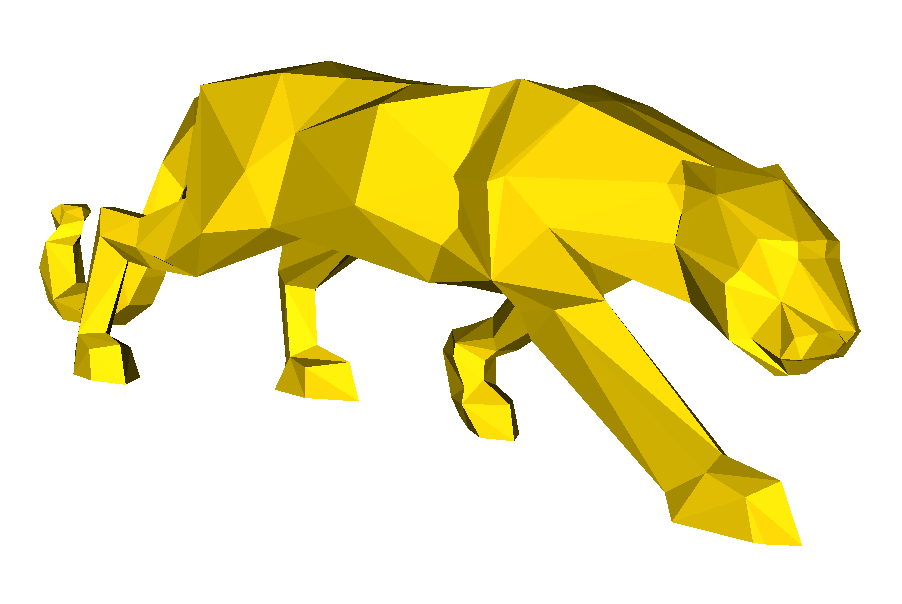
\includegraphics[width=3.5in]{images/pan_0.png}
    &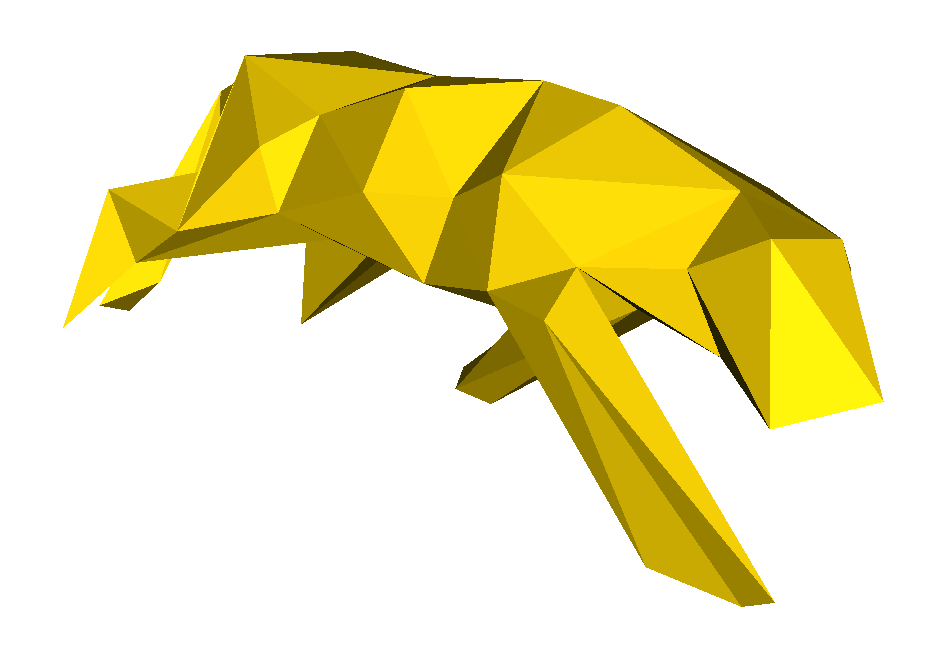
\includegraphics[width=3.5in]{images/pan_220.png}\\
    % $\begin{array}{@{\hspace{-0.00in}}c@{\hspace{0.05in}}c}
    % 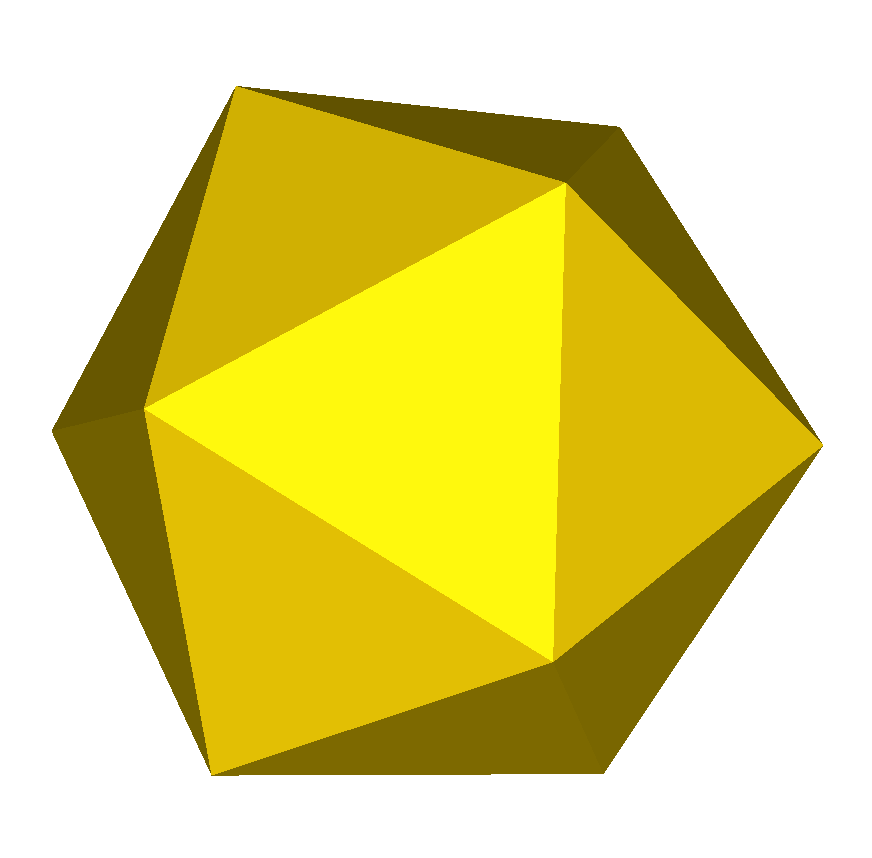
\includegraphics[height=1.3in]{images/ico_0.png}
    % &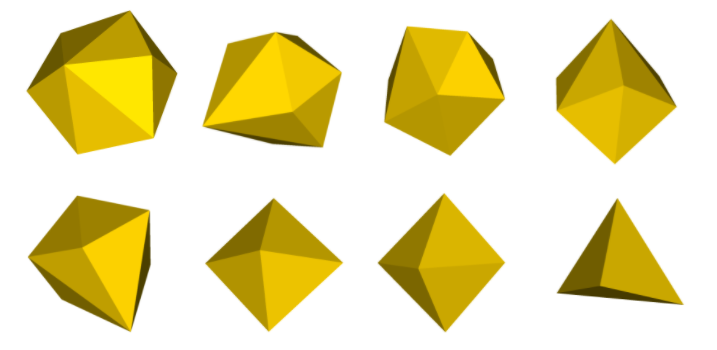
\includegraphics[height=1.3in]{images/ico_1-8.png}\\
    \end{array}$
\end{center}
\caption{Renderings of the original panther mesh with 570 faces and 287
vertices (left), and the result of applying our implementation of Garland and
Heckbert’s algorithm to the original panther for 220 contractions, producing a
new mesh with only 130 faces and 67 vertices (right).}
\label{fig:panther}
\end{figure*}

% SECTION Previous Work
desired, they developed their own algorithm based on iterative edge contraction
that can create high quality approximations of both manifold and non-manifold 
shapes with both speed and precision.
% !SECTION Previous Work

\section{Background}
% \label{sec:background}

% SECTION Results
\section{Results}
% \label{sec:results}
We implement the following pipeline for demonstrating Garland and Heckbert's
algorithm for surface simplification. % TODO cite
\begin{enumerate}
    \item Load a 3D model from a local PLY file, representing the faces and
    vertices as Python lists.
    \item Perform the necessary modifications to the vertices and faces, per
    the supplied command line parameters.
    \item Save the resulting mesh as a separate PLY file.
\end{enumerate}

Our small set of object models, curated from online academic sources and used
during development, spans many orders of magnitude in the number of initial
faces. Of these models, a typical, almost median-like sample was chosen as the
representative result to report. Figure~\ref{fig:panther} and those discussed in the % TODO figure...
following section were produced by our implementation. The transformative
effect of the algorithm manifests visually in this result in two key ways. Most
noticeably, the central mass of the model in the final model is composed of
many fewer triangular faces, than is the original. Moreover, the color and
shading of the rendering make it clear that the significant high-level features
of the model are clearly preserved with high fidelity (viz. the back haunch,
abdomen, shoulder).


% 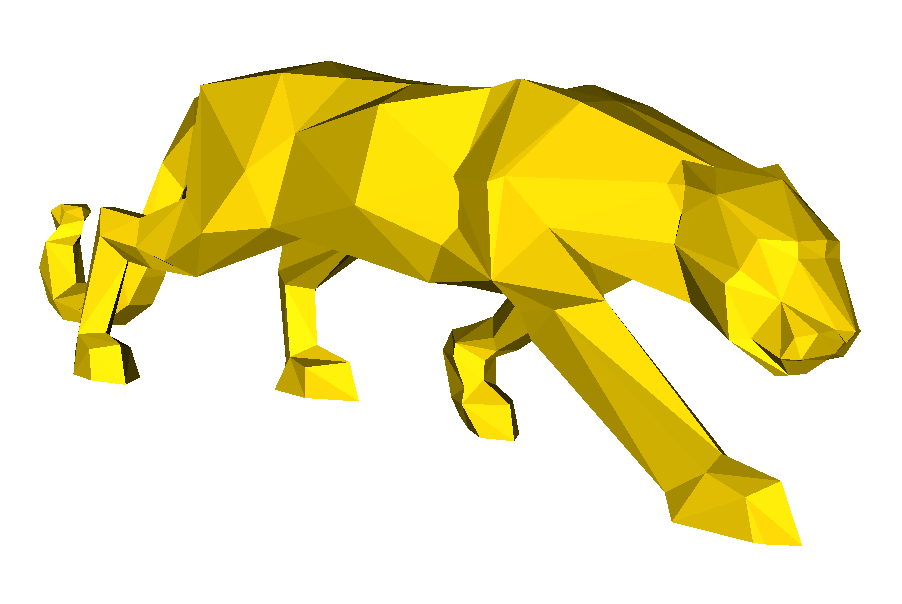
\includegraphics[height=1.3in]{images/pan_0.png}

% !SECTION Results

% SECTION Evaluation
\section{Evaluation}
% \label{sec:evaluation}
In their original paper, Garland and Heckbert give their method for
approximating error in the output mesh with respect to the original; this
method computes a heuristic for the spatial difference between the original and
final meshes. For our purposes of verifying functionality and correctness, we
chose to dispense with their purely quantitative method in the end, favoring a
more visualization-focused approach for evaluating efficacy to task. Conceptual
and mathematical constraints for a valid mesh state are enforced
programmatically via assert statements; to the extent that these assertions
accurately and comprehensively implement the constraints, the implementation
can be verified as correct through this means.

\subsection{Eyeball Test}
Ultimately, this algorithm and any implementation thereof is not useful unless
it is capable of producing visually pleasing models from the original. We
verified throughout development that our program effectively produces a
% “smooth” mesh with a reasonable degree of fidelity to the original [See panther].  % TODO
% However, it is difficult to observe the progressive influence of the algorithm on the appearance of the model when the original is of high-resolution; each contraction simply does not change the mesh enough to make those observations noticeable.

% \begin{figure*}[t]
% \begin{center}
%     $\begin{array}{@{\hspace{-0.00in}}c@{\hspace{0.05in}}c}
%     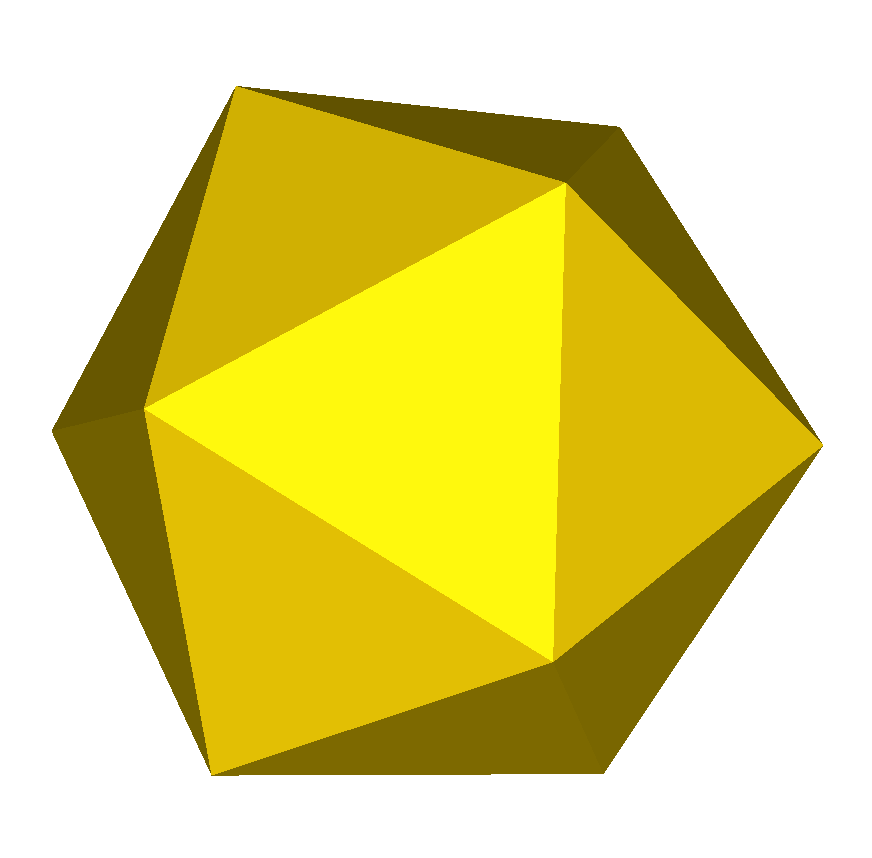
\includegraphics[height=1.3in]{images/ico_0.png}
%     &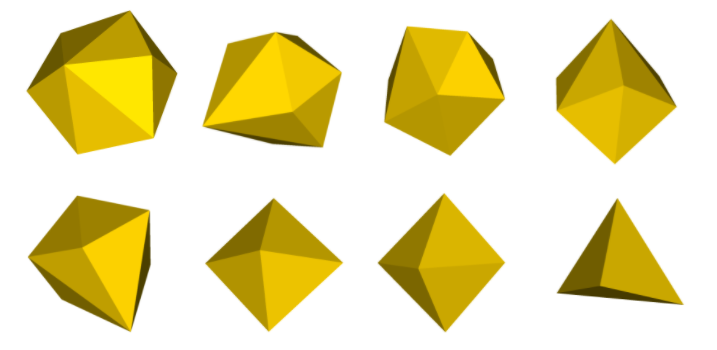
\includegraphics[height=1.3in]{images/ico_1-8.png}\\
%     % $\begin{array}{@{\hspace{-0.00in}}c@{\hspace{0.05in}}c}
%     % 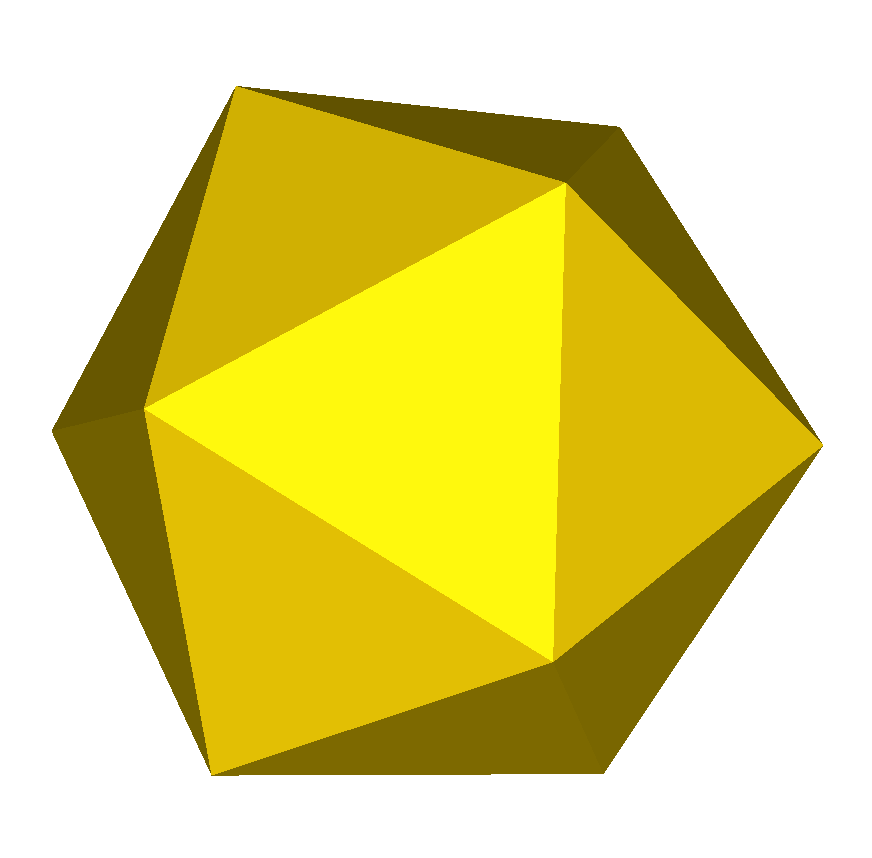
\includegraphics[height=1.3in]{images/ico_0.png}
%     % &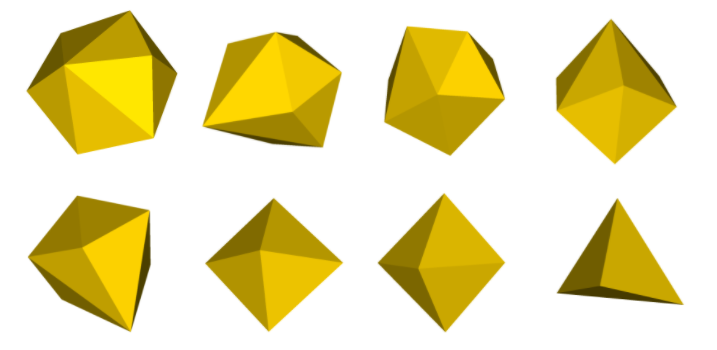
\includegraphics[height=1.3in]{images/ico_1-8.png}\\
%     \end{array}$
% \end{center}
% \caption{$N$-way rotational symmetries appear naturally in the
% Platonic solids: tetrahedron ($N=2$), octahedron ($N=3$), cube
% ($N=4$), icosahedron ($N=6$), and dodecahedron ($N=10$). }
% \label{fig:symmetry_examples}
% \end{figure*}

\subsection{Cost Analysis}

\subsection{Programmatic Assertions}
In order to ensure that our implementation is behaving as expected, it was
helpful at all stages of development to take advantage of Python’s built-in
\texttt{assert} statement to verify certain properties of our meshes 
mid-execution; this measure, of course, doubled as a means of diagnosing
sources of error in real-time. For example, we implement the constraint that,
following each contraction, no face is allowed to contain a vertex which has
already been contracted, removed. The relevant assert statements have been left
in the final implementation, variably commented out.
% !SECTION Evaluation

\section{Division of Tasks}
% \label{sec:division_of_tasks}
Tasks were divided up initially, but ultimately a lot of the bug fixing was done collaboratively. Jesse wrote the initial boilerplate code for steps 1-4 of the algorithm and put time into carefully selecting which Python libraries would be best suited for the algorithm and visualization. After a collaborative discussion on data structures, Odyssey reimplemented the boilerplate code into something that would better support the needs of step 5 of the algorithm. We worked together to get step 5 of the algorithm working and there was a lot of implementation and reimplementation until we had a working product.

% SECTION Conclusion
\section{Conclusion} % TODO
% \label{sec:Conclusion}

Our implementation of Garland and Heckbert’s algorithm demonstrates its
effectiveness in preserving high-level appearance while eliminating low-level
detail in 3D triangular meshes. However, if the preservation of vulnerable
semantic features (e.g. thin appendages in the resulting model) is essential
throughout surface simplification, then this algorithm should be applied with
caution and its outputs verified by eye for integrity to prevent similar
attenuation in customer-facing graphics. We further show that results can be
obtained via this algorithm in real time without the bare-metal speed promised
by C++, even in lieu of memoization a la dynamic programming.

% SECTION Conclusion

\end{document}
